\documentclass{article}
\usepackage[utf8]{inputenc}
\usepackage{amsmath, amssymb, amsthm}
\usepackage[margin=1in]{geometry}
\usepackage{graphicx}  % For including images
\usepackage{listings}  % For including code
\usepackage{xcolor}  % For code highlighting
\usepackage{subcaption}  % For subfigures
\usepackage{hyperref}
\usepackage{tikz}
\usepackage{pdfpages}
\usetikzlibrary{positioning}

% Define theorem environments
\newtheorem{theorem}{Theorem}
\newtheorem{lemma}{Lemma}
\newtheorem{definition}{Definition}
\newtheorem{corollary}{Corollary}
% Define custom solution environment
\newenvironment{solution}{\noindent\textbf{Solution:} }{\qed}
% Code listing style
\lstset{
    language=Python,
    basicstyle=\ttfamily\footnotesize,
    keywordstyle=\color{blue},
    commentstyle=\color{gray},
    stringstyle=\color{red},
    breaklines=true,
    numbers=left,
    numberstyle=\tiny\color{gray},
    frame=single
}
\usetikzlibrary{positioning, shapes, arrows.meta}

\title{ECE-GY 7143 Introduction to Deep Learning \\ \Large Homework 1}
\author{Ali Hamza (ah7072)}
\date{\today}

\begin{document}
\maketitle
\newpage
\section*{Question 1}
Given that a neuron is defined as follows:
\begin{equation}
    y = \sigma(w^T x + b) \quad \text{where} \quad \sigma(z) = \begin{cases}
        1 & \text{if } z > 0 \\
        0 & \text{otherwise}
    \end{cases}
\end{equation}
% and $y, x, w \in \mathbb{R}^1$ and $b \in \mathbb{R}$. The loss function is defined as:
% \begin{align}
%     L(y, \hat{y}) &= \frac{1}{2} (y - \hat{y})^2
% \end{align}
% \subsection*{Part (a)}
% \begin{solution}
% We can approximate the function of a box given by:
% \begin{equation}
%     f(x) = \begin{cases}
%         h & \text{if } 0 < x < \delta \\
%         0 & \text{otherwise}
%     \end{cases}
% \end{equation}
    
% \end{solution}
\subsection*{Part (a)}
We want to approximate the box function given by:
\[
f(x) = \begin{cases}
h & \text{if } 0 < x < \delta, \\
0 & \text{otherwise,}
\end{cases}
\]
using a neural network with two hidden neurons (defined above) and one linear output neuron. The neural network should output \( h \) only when \( 0 < x < \delta \), and 0 otherwise. We can achieve this by setting the weights and biases of the neurons as follows:
\begin{enumerate}
    \item \text{Input Layer:}  
          The input to the network is \( x \).
    \item \text{Hidden Layer:}
    \item \begin{enumerate}
        \item \text{Neuron 1:} Set weight \( w_1 = 1 \) and bias \( b_1 = 0 \) so that its pre-activation is
              \[
              z_1 = x,
              \]
              and its activation is 
              \[
              \sigma(z_1) = \sigma(x) = \begin{cases} 1, & x > 0 \\ 0, & x \le 0 \end{cases}.
              \]
        \item \text{Neuron 2:} Set weight \( w_2 = 1 \) and bias \( b_2 = -\delta \) so that its pre-activation is
                  \[
                  z_2 = x - \delta,
                  \]
                  and its activation is 
                  \[
                  \sigma(z_2) = \sigma(x-\delta) = \begin{cases} 1, & x > \delta \\ 0, & x \le \delta \end{cases}.
                  \]
    \end{enumerate}
    \item \text{Output Neuron:}  
          This neuron simply sums the weighted outputs of the hidden neurons without a nonlinearity. Set its weights as follows:
          \[
          \text{Weight on } \sigma(x):\quad h, \quad \text{and on } \sigma(x-\delta):\quad -h.
          \]
          Thus, the output is given by
          \[
          y = h\cdot \sigma(x) - h\cdot \sigma(x-\delta) = h\bigl[\sigma(x) - \sigma(x-\delta)\bigr].
          \]
\end{enumerate}
\begin{center}
\begin{tikzpicture}[>=stealth, node distance=2cm, auto]

    % Input node
    \node[draw, rectangle, minimum width=1cm, minimum height=1cm] (input) {$x$};
    
    % Hidden layer nodes
    \node[draw, circle, right=of input, minimum size=1cm] (h1) {$n_1$};
    \node[draw, circle, below=of h1, minimum size=1cm] (h2) {$n_2$};
    
    % Output node
    \node[draw, rectangle, right=of h1, minimum width=1cm, minimum height=1cm] (output) {$y$};
    
    % Connections: input to hidden layer
    \draw[->] (input) -- (h1);
    \draw[->] (input) -- (h2);
    
    % Connections: hidden layer to output
    \draw[->] (h1) -- node[above] {\(h\)} (output);
    \draw[->] (h2) -- node[below] {\(-h\)} (output);
    
\end{tikzpicture}
\end{center}

\textbf{Cases:}
\begin{enumerate}
    \item For \( x < 0 \):  
          \(\sigma(x) = 0\) and \(\sigma(x-\delta) = 0\) (since \(x-\delta < 0\)), hence
          \[
          y = h\,(0 - 0) = 0.
          \]
    \item For \( 0 < x < \delta \):  
          \(\sigma(x) = 1\) (since \(x > 0\)) and \(\sigma(x-\delta) = 0\) (since \(x-\delta < 0\)), hence
          \[
          y = h\,(1 - 0) = h.
          \]
    \item For \( x > \delta \):  
          \(\sigma(x) = 1\) and \(\sigma(x-\delta) = 1\) (since \(x-\delta > 0\)), hence
          \[
          y = h\,(1 - 1) = 0.
          \]
\end{enumerate}
Thus, the network outputs \( h \) only when \( 0 < x < \delta \), perfectly recreating the desired box function.

\subsection*{Part (b)}
We wish to approximate a smooth, bounded function 
\[
f: [-B,B] \to \mathbb{R},
\]
by representing it as a sum of simple “box functions” that are easy to implement in a neural network. The idea is analogous to forming a Riemann sum.

\noindent\textbf{Step 1: Partitioning the Domain}\\[0.5em]
Divide the interval \([-B,B]\) into \(N\) small subintervals of equal width
\[
\delta = \frac{2B}{N}.
\]
Label the endpoints as
\[
x_i = -B + i\delta, \quad \text{for } i = 0, 1, \dots, N.
\]
Over each interval \([x_i, x_i+\delta]\), the function \( f(x) \) does not vary much, so we approximate it by a constant value
\[
c_i = f\Bigl(x_i + \frac{\delta}{2}\Bigr),
\]
which is the function value at the midpoint.

\noindent\textbf{Step 2: Representing \(f\) as a Sum of Box Functions}\\[0.5em]
Define the indicator (or box) function for the \(i\)th subinterval as:
\[
\chi_{[x_i,x_i+\delta]}(x) =
\begin{cases}
1, & \text{if } x \in [x_i, x_i+\delta],\\[1mm]
0, & \text{otherwise.}
\end{cases}
\]
Then \(f\) is approximated by the piecewise constant function:
\[
f_{\text{approx}}(x) = \sum_{i=0}^{N-1} c_i\, \chi_{[x_i,x_i+\delta]}(x).
\]
This is very similar to the idea behind Riemann sums, where you sum the contributions of small “rectangles” to approximate a function.

\noindent\textbf{Step 3: Realizing Box Functions in a Neural Network}\\[0.5em]
From Part (a) we saw a single box function on an interval \([a, a+\delta]\) can be implemented using two neurons with step activation functions:
\begin{itemize}
    \item \textbf{Neuron 1:} Computes \(\sigma(x - a)\). It outputs 1 when \(x > a\) (thus “turning on” the box at the left edge).
    \item \textbf{Neuron 2:} Computes \(\sigma(x - (a+\delta))\). It outputs 1 when \(x > a+\delta\) (thus “turning off” the box at the right edge).
\end{itemize}
Taking the difference,
\[
\sigma(x - a) - \sigma(x - (a+\delta)),
\]
produces 1 exactly when \(x \in (a, a+\delta)\) and 0 otherwise. Multiplying by \(c_i\) scales the box function to the appropriate height.

\bigskip
\noindent\textbf{Step 4: Combining the Boxes in the Network}\\[0.5em]
The overall network approximates \(f(x)\) by summing over the outputs of all these box detectors:
\[
y(x) = \sum_{i=0}^{N-1} c_i \left[ \sigma(x-x_i) - \sigma(x-(x_i+\delta)) \right].
\]
As we make \(\delta\) smaller (i.e., increasing \(N\)), the sum becomes a closer approximation to \(f(x)\). We can show the neural network as follows:
\bigskip
\begin{center}
    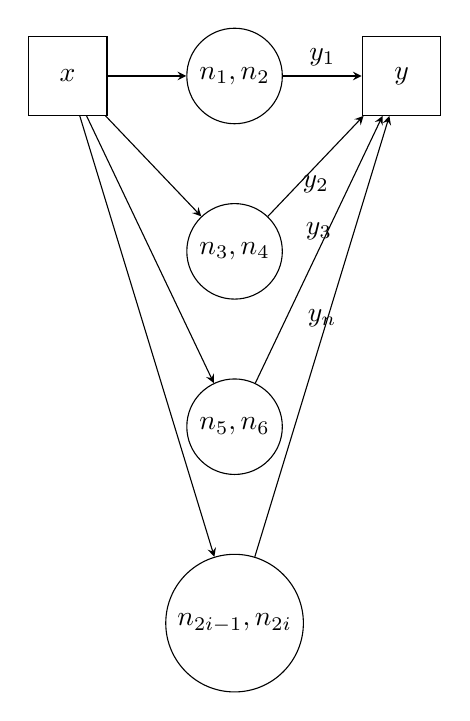
\begin{tikzpicture}[>=stealth, node distance=1cm, auto]
    
        % Input node
        \node[draw, rectangle, minimum width=1cm, minimum height=1cm] (input) {$x$};
        
        % Hidden layer nodes
        \node[draw, circle, right=of input] (h1) {$n_1, n_2$};
        \node[draw, circle, below=of h1] (h2) {$n_3, n_4$};
        \node[draw, circle, below=of h2] (h3) {$n_5, n_6$};
        \node[draw, circle, below=of h3] (h4) {$n_{2i-1}, n_{2i}$};
        
        % Output node
        \node[draw, rectangle, right=of h1, minimum width=1cm, minimum height=1cm] (output) {$y$};
        
        % Connections: input to hidden layer
        \draw[->] (input) -- (h1);
        \draw[->] (input) -- (h2);
        \draw[->] (input) -- (h3);
        \draw[->] (input) -- (h4);
        
        % Connections: hidden layer to output
        \draw[->] (h1) -- node[above] {\(y_1\)} (output);
        \draw[->] (h2) -- node[below] {\(y_2\)} (output);
        \draw[->] (h3) -- node[above] {\(y_3\)} (output);
        \draw[->] (h4) -- node[above] {\(y_n\)} (output);
        
    \end{tikzpicture}
    \end{center}
Where each pair of neurons \((n_{2i-1}, n_{2i})\) implements a box function over the interval \([x_i, x_i+\delta]\) as described in Part (a) and the output neuron sums the contributions from all these pairs.
\subsection*{Part (c)}

The same construction extends to functions \( f: \mathbb{R}^d \to \mathbb{R} \) by partitioning a bounded region in \( \mathbb{R}^d \) into many small \(d\)-dimensional boxes (hyperrectangles).

\begin{itemize}
    \item Partition each dimension into \(N\) segments, creating \(N^d\) hyperrectangles.
    \item For each hyperrectangle \( R \), define an indicator function
    \[
    \chi_R(x) =
    \begin{cases}
    1, & \text{if } x \in R,\\[1mm]
    0, & \text{otherwise.}
    \end{cases}
    \]
    \item Approximate \( f(x) \) by summing over these boxes:
    \[
    f_{\text{approx}}(x) = \sum_R c_R\, \chi_R(x),
    \]
    where \( c_R \) is chosen to approximate \( f \) in that region.
\end{itemize}
The number of boxes grows exponentially with \( d \) (i.e., \(N^d\)). This means that while the method is theoretically sound, the neural network would require an impractically large number of neurons in high-dimensional settings.

\newpage
\section*{Question 2}

Given a  single fully-connected layer with $n_{\text{in}}$ inputs and $n_{\text{out}}$ outputs. Each weight $W_{ji}$ is drawn from a Gaussian distribution $\mathcal{N}(0, \sigma^2)$, and the biases are zero. The inputs $x_i$ are i.i.d.\ with mean 0 and variance $v^2$. We want to find constraints on $\sigma^2$ so that the variance of the neuron outputs does not vanish or explode, and similarly for the backward pass gradients.
\subsection*{Part (a)}
Consider a single neuron's output:
\[
a_j = \sum_{i=1}^{n_{\text{in}}} W_{ji}\, x_i.
\]
Since $W_{ji} \sim \mathcal{N}(0, \sigma^2)$ and $x_i$ are i.i.d.\ with $\mathrm{Var}(x_i) = v^2$,
\[
\mathbb{E}[a_j] = 0, 
\]
and
\[
\mathrm{Var}(a_j) \;=\; \mathbb{E}\Bigl[a_j^2\Bigr] 
\;=\; \sum_{i=1}^{n_{\text{in}}} \mathbb{E}\bigl[W_{ji}^2\, x_i^2\bigr]
\;=\; \sum_{i=1}^{n_{\text{in}}} \bigl(\mathbb{E}[W_{ji}^2]\bigr)\,\bigl(\mathbb{E}[x_i^2]\bigr)
\;=\; n_{\text{in}}\;\sigma^2\;v^2.
\]

\subsection*{Part (b)}
If $\sigma^2$ is too large, $\mathrm{Var}(a_j)$ grows with $n_{\text{in}}$, leading to exploding activations. If $\sigma^2$ is too small, the variance goes to zero with increasing $n_{\text{in}}$. A rough rule to keep the variance at a stable scale is:
\[
n_{\text{in}}\;\sigma^2 \approx 1 
\quad\Longrightarrow\quad 
\sigma^2 \approx \frac{1}{n_{\text{in}}}.
\]

\subsection*{Part (c)}
If the neuron has a ReLU activation, only about half of the inputs (on average) will be positive (assuming a symmetric distribution around 0). This halves the effective variance. Hence, to preserve variance across a ReLU, we need:
\[
\frac{1}{2}\,n_{\text{in}}\;\sigma^2 \approx 1
\quad\Longrightarrow\quad
\sigma^2 \approx \frac{2}{n_{\text{in}}}.
\]
Thus, compared to the linear case, the initialization variance is scaled by a factor of 2.

\subsection*{Part (d)}
During backpropagation, gradients to the input layer are computed via
\[
\delta_{\text{in}} = W^T\,\delta_{\text{out}},
\]
where $\delta_{\text{out}}$ has variance $g^2$. A similar derivation shows that
\[
\mathrm{Var}(\delta_{\text{in}}) \;=\; n_{\text{out}}\,\sigma^2\,g^2.
\]
To avoid exploding or vanishing gradients, we also need
\[
n_{\text{out}}\,\sigma^2 \approx 1 
\quad\Longrightarrow\quad
\sigma^2 \approx \frac{1}{n_{\text{out}}}.
\]

\subsection*{Part (e)}
To balance both forward and backward stability, we want $\sigma^2$ to be on the order of both $1/n_{\text{in}}$ and $1/n_{\text{out}}$. A reasonable choice is the harmonic mean of the two:
\[
\sigma^2 \approx \frac{2}{n_{\text{in}} + n_{\text{out}}}.
\]
To account for the ReLU activation, we scale this by a factor of 2:
\[
\sigma^2 \approx \frac{4}{n_{\text{in}} + n_{\text{out}}}.
\]

% \newpage
% \section*{Question 3}
% The FashionMNIST classifier was improved by replacing the simple logistic regression (a single linear layer) with a deeper network containing three fully connected hidden layers with 256, 128, and 64 neurons, respectively, each followed by a ReLU activation. The network architecture is as follows:

% \begin{enumerate}
%     \item \textbf{Input Layer:}  
%           The input layer has 784 neurons corresponding to the 28x28 image pixels.
%     \item \textbf{Hidden Layer 1:}
%     \begin{enumerate}
%         \item \textbf{Fully Connected Layer:}  
%               This layer has 256 neurons and applies a linear transformation to the input followed by a ReLU activation.
%         \item \textbf{Activation:}  
%               The ReLU activation function is applied element-wise to the output of the fully connected layer.

%         \end{enumerate}
%     \item \textbf{Hidden Layer 2:}
%     \begin{enumerate}
%         \item \textbf{Fully Connected Layer:}  
%               This layer has 128 neurons and applies a linear transformation to the input followed by a ReLU activation.
%         \item \textbf{Activation:}  
%               The ReLU activation function is applied element-wise to the output of the fully connected layer.

%         \end{enumerate}
%     \item \textbf{Hidden Layer 3:}
%     \begin{enumerate}
%         \item \textbf{Fully Connected Layer:}  
%               This layer has 64 neurons and applies a linear transformation to the input followed by a ReLU activation.
%         \item \textbf{Activation:}  
%               The ReLU activation function is applied element-wise to the output of the fully connected layer.

%         \end{enumerate}
%     \item \textbf{Output Layer:}  
%           The output layer has 10 neurons corresponding to the 10 classes in FashionMNIST. It applies a linear transformation to the input followed by a softmax activation.

% \end{enumerate}

% The network using the SGD optimizer (learning rate = 0.001) and CrossEntropyLoss over 20 epochs. During training, both the training and test losses were recorded, as well as the test accuracy. The following observations were made:

% The training loss decreases steadily over the epochs, indicating that the network is learning the training data well. The test loss also decreases initially but starts to increase slightly after epoch 10. This suggests that the model may be overfitting the training data. The test accuracy reaches 85.82\%, and the minimimum test loss i 0.3954
% indicating that the model is generalizing well to unseen data. The linear regression model achieved minimum train loss of 0.4515 and test loss 0.4849. The full training and test loss curves are shown in Figure \ref{fig:loss_1} and Figure \ref{fig:loss} for the logistic regression and deep network models, respectively.
% \begin{figure}[h!]
%     \centering
%     \begin{subfigure}[b]{0.45\textwidth}
%         \includegraphics[width=\textwidth]{loss_1.png}
%         \caption{Logistic Regression}
%         \label{fig:loss_1}
%     \end{subfigure}
%     \begin{subfigure}[b]{0.45\textwidth}
%         \includegraphics[width=\textwidth]{loss.png}
%         \caption{Deep Network}
%         \label{fig:loss}
%     \end{subfigure}
%     \caption{Training and Test Loss Curves for Logistic Regression and Deep Network Models}
% \end{figure}

% We can see that the deep network model achieves a lower test loss and higher test accuracy compared to the logistic regression model. This indicates that the deep network is better able to capture the complex patterns in the FashionMNIST dataset, leading to improved performance. The model was also used to make predictions on randomly selected images from the test set (Figure \ref{fig:predictions}). 
% % 3 images stacked vertically
% \begin{figure}[h!]
%     \centering
%     \begin{subfigure}[b]{0.3\textwidth}
%         \includegraphics[width=\textwidth]{output_1.png}
%     \end{subfigure}
%     \begin{subfigure}[b]{0.3\textwidth}
%         \includegraphics[width=\textwidth]{output_2.png}
%     \end{subfigure}
%     \begin{subfigure}[b]{0.3\textwidth}
%         \includegraphics[width=\textwidth]{output_3.png}
%     \end{subfigure}
%     \caption{Deep Network Predictions on 3 Random Test Images}
%     \label{fig:predictions}
% \end{figure}

% For most images, the model assigns a high probability to the correct class. However, there are some cases where the model is less confident, such as the third image where the image is more complex and contains multiple patterns that could belong to different classes. Overall, the deep network model demonstrates good performance on the FashionMNIST dataset, achieving a test accuracy of $\approx$ 85\%.
% \includepdf[pages=-]{demo01-basics.pdf} 

\newpage
\section*{Question 3}

We improved the FashionMNIST classifier by replacing a simple logistic regression (a single linear layer) with a deeper network. The new architecture comprises three fully connected hidden layers with 256, 128, and 64 neurons, each followed by a ReLU activation. The details are as follows:

\begin{enumerate}
    \item \textbf{Input Layer:}  
          784 neurons (28$\times$28 image pixels).
    \item \textbf{Hidden Layer 1:}
          \begin{enumerate}
              \item Fully Connected layer with 256 neurons.
              \item ReLU activation.
          \end{enumerate}
    \item \textbf{Hidden Layer 2:}
          \begin{enumerate}
              \item Fully Connected layer with 128 neurons.
              \item ReLU activation.
          \end{enumerate}
    \item \textbf{Hidden Layer 3:}
          \begin{enumerate}
              \item Fully Connected layer with 64 neurons.
              \item ReLU activation.
          \end{enumerate}
    \item \textbf{Output Layer:}  
          Fully connected layer with 10 neurons (one per class) followed by softmax activation.
\end{enumerate}

The network was trained using the SGD optimizer (learning rate = 0.001) and CrossEntropyLoss for 20 epochs. The training loss decreased steadily, while the test loss decreased initially and then slightly increased after epoch 10, suggesting some overfitting. The deep network achieved a minimum test loss of 0.3954 and a test accuracy of 85.82\%, compared to the logistic regression model’s training loss of 0.4515 and test loss of 0.4849.

Figures \ref{fig:loss_1} and \ref{fig:loss} display the loss curves for the logistic regression and deep network models, respectively.

\begin{figure}[h!]
    \centering
    \begin{subfigure}[b]{0.45\textwidth}
        \includegraphics[width=\textwidth]{loss_1.png}
        \caption{Logistic Regression}
        \label{fig:loss_1}
    \end{subfigure}
    \begin{subfigure}[b]{0.45\textwidth}
        \includegraphics[width=\textwidth]{loss.png}
        \caption{Deep Network}
        \label{fig:loss}
    \end{subfigure}
    \caption{Training and Test Loss Curves}
\end{figure}

Additionally, predictions on random test images show that the model generally assigns a high probability to the correct class. However, for more complex images with multiple patterns, the confidence is reduced.

Overall, the deep network more effectively captures complex patterns in the FashionMNIST dataset, leading to better generalization and performance compared to logistic regression.

\includepdf[pages=-]{demo01-basics.pdf}

\newpage
\section*{Question 4}
The general structure of the Python Notebook for this question is as follows:
\begin{enumerate}
    \item Load MNIST dataset using using TensorFlow, and show some sample images.
    \item Define \texttt{sigmoid, dsigmoid, softmax, cross\_entropy\_loss} functions.
    \item Network setup
    \begin{itemize}
        \item Two layer neural network with 784 input neurons, 128 hidden neurons, and 10 output neurons.
        \item Global list of weights and biases for each layer initialized using gaussian distribution.
    \end{itemize}
    \item Feedforward and backpropagation functions.
    \begin{itemize}
        \item \texttt{feed\_forward\_sample} computes the activations and returns the loss and one-hot prediction for a single sample.
        \item \texttt{feed\_forward\_dataset} applies the sample function over all data and reports average loss and accuracy.
        \item  \texttt{train\_one\_sample}performs a forward pass, computes the loss, then backpropagates errors to compute gradients.
        \item Gradients are computed using the chain rule, and the parameters are updated accordingly.
    \end{itemize}
    \item Training the network
        \begin{itemize}
        \item \texttt{train\_one\_epoch} loops through every training sample 
        \item \texttt{test\_and\_train} runs an epoch then evaluates on the test set.
    \end{itemize}
\end{enumerate}

\includepdf[pages=-]{hw1_s25_p4.pdf}

\section*{References}

\begin{enumerate}
    \item \href{https://d2l.ai/chapter_linear-classification/index.html}{4. Linear Neural Networks for Classification}
    \item \href{https://d2l.ai/chapter_multilayer-perceptrons/index.html}{5. Multilayer Perceptrons}
    \item GPT O3 used for syntax referencing, report formatting, and general guidance backpropagation.
    \item Discussed solutions, concepts, and ideas with Saad Zubairi
\end{enumerate}



\end{document}